%preamble
%%%%%%%%%%%

\documentclass[a4paper, 11pt]{article}


% TODO s:
%            - Table of contents
%            - Taakverdeling duidelijker

%Packages gebruiken
%%%%%%%%%%%%%%%%%%%%%

\usepackage[dutch]{babel} % Voor nederlandstalige hyphenatie
\usepackage{amsmath} % Uitgebreide wiskundige mogelijkheden
\usepackage{url} % Om url�s te verwerken 
	%bv: \url{http://zeus.ugent.be/} geeft http://zeus.ugent.be/.
\usepackage[latin1]{inputenc} % Om niet ascii karakters te kunnen typen
	%bv: ��� ...

% Volgend package is niet echt nodig. Het laat echter toe om gemakkelijk elektronisch
% te navigeren in je pdf-document. Deze package moet altijd als laatste ingeladen worden.
\usepackage[a4paper,plainpages=false]{hyperref}    % Om hyperlinks te hebben in het pdfdocument.

%Hack om bibliografische referenties te kunnen doen
%Gevonden op: http://www.kronto.org/thesis/tips/url-formatting.html
%% Define a new 'leo' style for the package that will use a smaller font.
\makeatletter
\def\url@leostyle{%
  \@ifundefined{selectfont}{\def\UrlFont{\sf}}{\def\UrlFont{\small\ttfamily}}}
\makeatother
%% Now actually use the newly defined style.
\urlstyle{leo}

%voor het weergeven van code
\usepackage{listings}
%settings voor code listings
\lstset{
	basicstyle=\small,
	tabsize = 2,
	language = [Sharp]C}

%Afbeeldingen in pdf formaat
\usepackage{epsfig}
\usepackage{graphicx}
\DeclareGraphicsExtensions{.pdf}

% PDF specifieke opties.
% Is hetgeen verschijnt wanneer je in acroread de documentproperties bekijkt.
\hypersetup{
    pdfauthor = {Jonathan Slendes en Christophe Lambrechts},
    pdftitle = {Trimester overschreidend project - .NET YAML Parser},
    pdfsubject = {Analyse verslag},
    pdfkeywords = {Trimester overschreidend project, YAML, Parser, Groeps project, .NET, C}
}

%nieuwe commando's
%%%%%%%%%%%%%%%%%%%%%


%hoofding
%%%%%%%%%%

\date{\today}
\title{Trimester overschreidend project \\ .NET YAML Parser}
\author{Jonathan~Slenders\and Christophe~Lambrechts}

%begin document
%%%%%%%%%%%%%%%%

\begin{document}

\maketitle

%samenvatting
%\begin{abstract}

In dit analyse verslag zullen we enerzijds trachten te schetsen wat onze doelstellingen zijn en anderzijds hoe 
wij ons het verloop van het project voorstellen. In dit vroege stadium is het bijzonder moeilijk om een volledig
overzicht te hebben op het project. Dit temeer door de volledig nieuwe domeinen die we moeten verkennen, zoals de mark-up taal 
YAML, de programmeer taal C\#, de ontwikkeling van een library voor opensource doeleinden, \ldots

%\end{abstract}

\section{Opgave}
YAML \footnote{YAML Ain't Markup Language} \cite{YHome} is een zeer leesbaar en makkelijk te bewerken data serialisatieformaat. 
Het kan gezien worden als een light-weight alternatief voor XML. YAML is opgebouwd rond het idee dat alle data 
voorgesteld kan worden met combinaties van lijsten, hashtables en scalaire data. YAML kan makkelijk gemapt worden 
op data types van de meeste high-level programmeertalen. Voor een korte inleiding kan je al eens 
kijken naar Yaml in Five Minutes \cite{Y5min}. Het YAML Cookbook illustreert hoe YAML's datastructuren mappen op die van Ruby \cite{YCookbook}.
 Er zijn parsers beschikbaar voor scripting talen zoals Python, PHP, Perl en Ruby, alsook een Java implementatie \cite{Yjava}. 
Ruby gebruikt YAML zelfs als het standaard serialisatieformaat. Deze implementaties gebruiken vaak onderliggend ook Syck \cite{Ysyck},
 een snelle implementatie in C. \label{opgave} Voor het .NET platform is er echter nog geen native parser beschikbaar. 
De studenten doen ervaring op met het .NET framework en de programmeertaal C\# en leren een specificatie te 
bestuderen en te implementeren. Het is de bedoeling het uiteindelijke resultaat als een open source library 
vrij te geven. 

\newpage

\section{Contact personen}

\begin{itemize}
\item Jo Vermeulen (\url{jo.vermeulen@uhasselt.be})
\item Tom Van Laerhoven (\url{tom.vanlaerhoven@uhasselt.be})
\end{itemize}


\section{Diepgaande beschrijving van het onderwerp}
Zoals reeds vermeld in de opgave (sectie \ref{opgave}), zullen we een parser implementeren in C\# voor YAML (klinkt als 'camel').
We zullen ons baseren op bestaande parser in Ruby die gebruik maakt van Syck. Dit houdt in dat we trachten in grote
maten de toegang tot de library en de functies te uniformeren. Bij de implementatie van het project zullen we van nul beginnen.
De hoofddoelstelling is propere en goed leesbare code te schrijven via de object-ge\"oorienteerde principes van C\#, dit in
tegenstelling tot Syck, die sterk is geoptimaliseerd, met als nadeel dat men moet in boeten tegen netheid en leesbaarheid.
Syck gebruikt bijvoorbeeld veel sprong instructies, iets wat sterk indruist tegen een goede programeer stijl.
C\# is een sterk objectgeori\"enteerde taal, we zullen dus steeds zoveel mogelijk van deze OO-structuren gebruik maken.

Bij het ontwerp van de parser zullen we zoveel mogelijk de offici\"ele YAML 1.1 specificatie \cite{YSpec} volgen.
We stellen echter niet als doel deze volledig te realiseren, temeer omdat er momenteel discussies op gang zijn gekomen
om YAML te vereenvoudigen. De belangrijkste elementen zullen uiteraard werken, later kunnnen nog details worden toegevoegd.

Onze Parser zal uit twee delen bestaan. Ten eerste kan deze YAML bestanden inlezen uit een bestand (of uit een string)
en vervolgends \emph{parsen}. Ten tweede zal deze ook een gecre\"eerde of geweizigde datastructuur terug naar een YAML-bestand
(of naar een string) kunnen uitschrijven (\emph{generator}).

Verder zullen we ook een beperkte test applicatie schrijven waarbij eenvoudig de werking van de parser ge\"evalueerd kan worden.
Vanzelfsprekend voorzien we in een set van voorbeeld YAML documenten. Om ook het praktische nut te kunnen aantonen van YAML
zullen we onze activiteiten logs en onderlinge communicatie opmaken in YAML.

Buiten deze technische details willen we ook graag aandacht vestigen op andere aspecten van programmeer projecten.
Zo gebruiken we CVS om code en project gerelateerde documenten te centraliseren. De ingebouwde documentatie mogelijkheden
van C\# en het .NET Framework, gebaseerd op XML zullen we benutten, dit ter vervanging van Doxygen in eerdere projecten.
De 'automatisch' gegenereerde documentatie zal ook van pas komen in het opensource aspect van dit project.
We zijn ons er echter van bewust dat deze nooit volledig is en enkel een hulp biedt voor de developpers. We zullen de
documentatie daarom uitbreiden met een eigen handleiding. Om het opensource project zoveel mogelijk kansen te bieden
zullen we trachten de code compatibel te maken met zowel het .NET Framework (Windows) als met Mono (voor Linux, Mac OS, ...).
Mogelijk zal deze ook in het .NET Compact Framework werken.


\section{Analyse}
	\subsection{Klasse-diagram}
	
\begin{figure}[hbt]
	\centering
		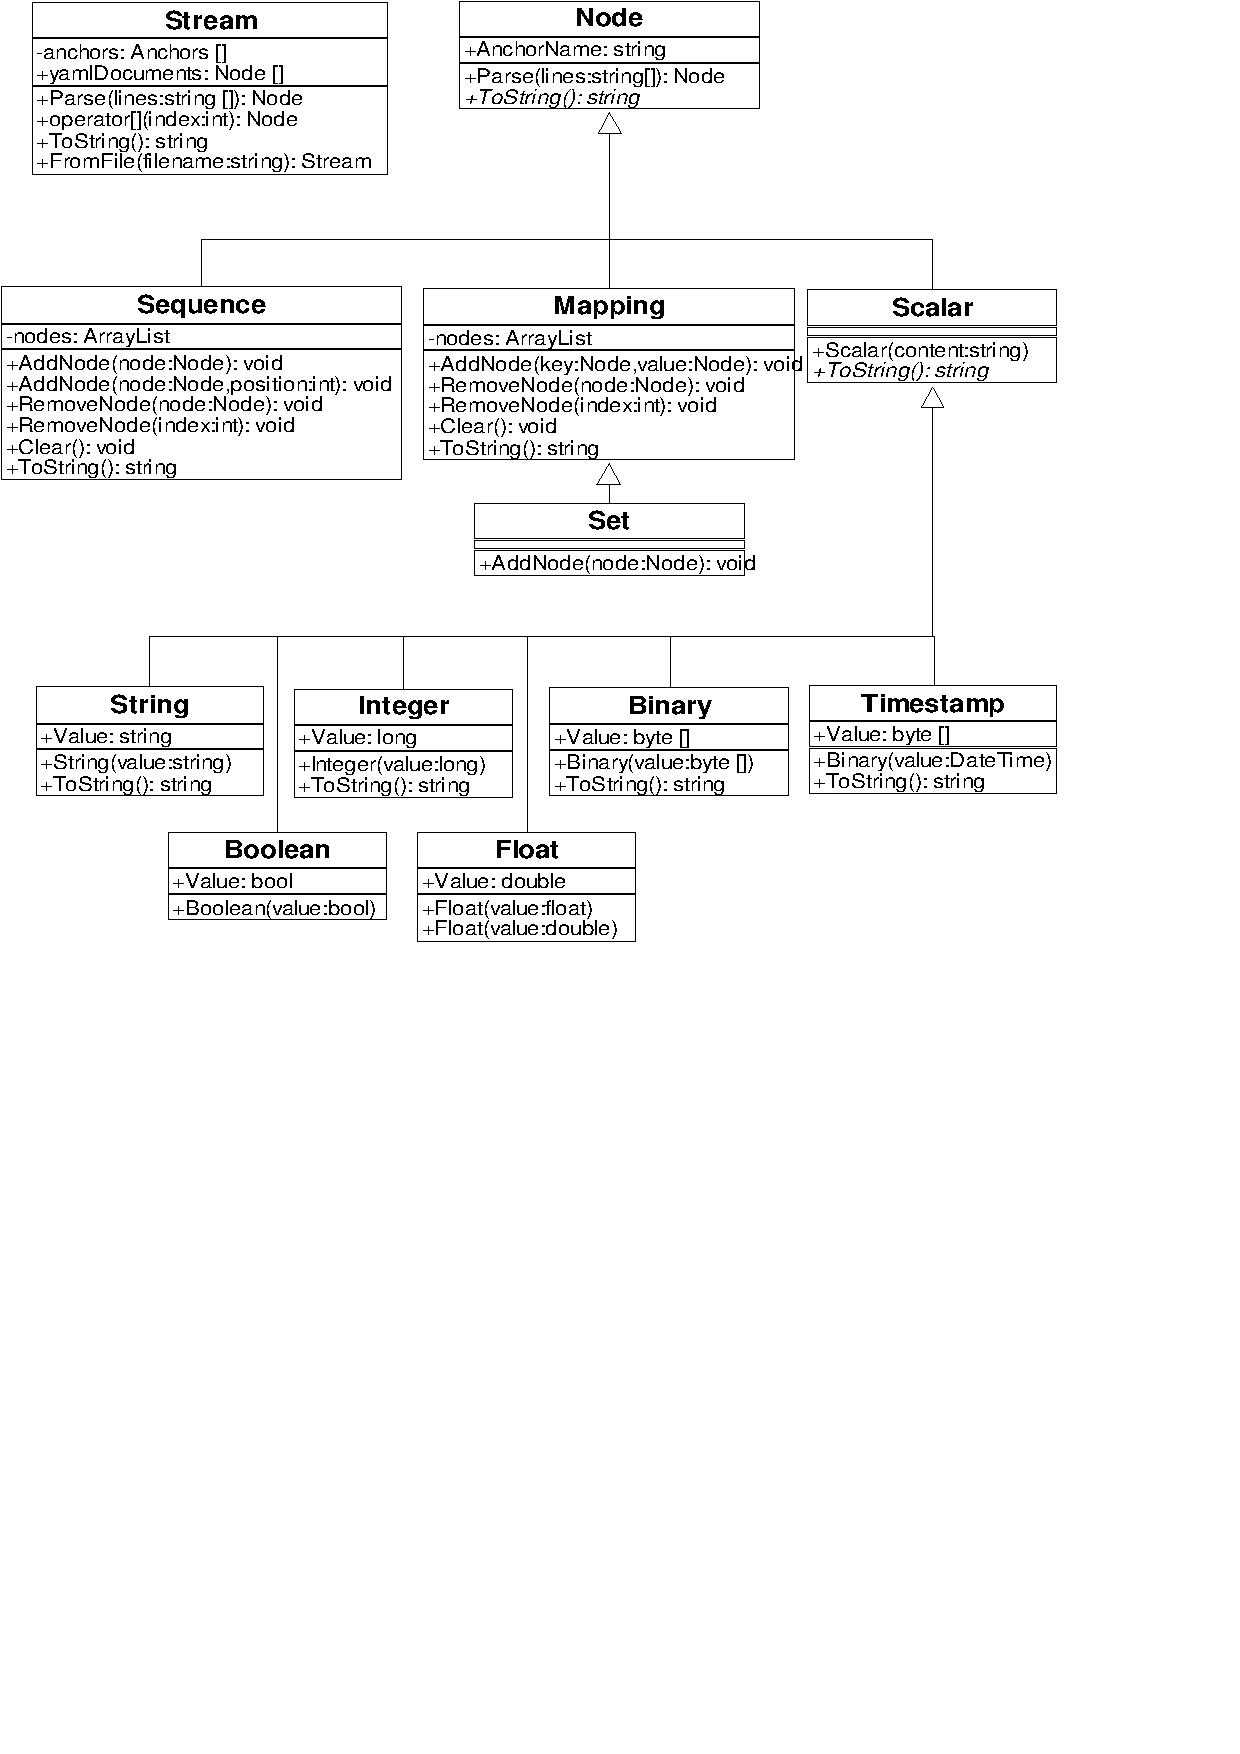
\includegraphics[width=1\textwidth]{uml.pdf}
	\caption{UML diagram voor YAML .NET Parser}
	\label{fig:UML}
\end{figure}
	
	Buiten de algemene boomstructuur merken we ook een \emph{stream} classe die eigenlijk de toegang is voor de gebruiker.
	Belangrijk is hierbij op te merken dat er zowel 'communicatie' mogelijk is via file I/O als via strings.
	
	Verder zijn de classe voor de test applicatie hier niet gerepresenteerd. Deze zullen minimaal van opbouw zijn en behoren
	strikt gezien ook niet tot de parser.

	\subsection{Verantwoording van de keuze van ADT's}

		\subsubsection{Algemene datastructuur}
		Onze datastructuur van een YAML document zal uit een boom van nodes bestaan. De wortel is het YAML document zelf,
		dit kan een mapping, sequence of scalar zijn. (Een bestand kan meerdere YAML documenten bevatten, in dat geval hebben
		we een ArrayList\footnote{het .NET alternatief voor een vector} van documenten.

		Elk element wordt voorgesteld door een classe die van de class \emph{Node} erft. In het geval
		van een \emph{Mapping} zal elk item in een ArrayList opgeslagen worden waarbij voor elk item zowel een key
		als de data gespecifieerd worden. Zowel de key als de data kan eender welk type \emph{Node} zijn, zelfs een andere \emph{Mapping}.

		Een \emph{Sequence} zal ook opgeslagen worden als ArrayList, maar in dit geval is er enkel een value, ook van het
		type \emph{Node}. \emph{Scalars} zijn primaire types, de bladeren van de boom, deze erven wel van \emph{Node}, maar kunnen zelf
		geen kinderen hebben. We gaan verschillende klassen gebruiken die van \emph{Scalar} erven, om onder andere types zoals
		date, string en numerieke waarden te implementeren.

		Verder kent YAML ook aliassen en anchor. Om deze voor te stellen zullen we gebruik maken van references naar objecten.
		De container die onze YAML documenten gaat bevatten zal een lijst van anchors bewaren, deze lijst gaat enkel gebruikt
		worden tijdens het parsen om latere aliasen te koppelen aan eerder gedefinieerde anchors. Na het parsen zal dat door
		een referentie (object referentie van C\#) in de boomstructuur worden vervangen.  Om er voor te zorgen dat men ook
		de originele YAML file kan reconstrueren, voorzien we in elke node een veld om de naam op te slaan van het
		mogelijke anchor.
		
		% Verder zal het ook nodig zijn dat we een waarde voorzien die zegt of een reference naar een node een anchor
		% of een alias is, dit om onnodige dubbels te voorkomen bij het wegschrijven van een YAML document.

	\subsection{Algoritmes}

		Dit zijn slechts grove lijnen van hoe we denken de algemene structuur te parsen. We zullen trachten een one-pass
		parser te maken, vermits bij het ontwerpen van YAML hier extra aandacht aan besteed werd. Het maakt de
		implementatie misschien niet alleen eenvoudiger, maar ook sneller.  De latere implementatie kan mogelijk
		afwijken omwille van een beter inzicht in de structuur die aantoont dat een ander algoritme effici\"enter is
		of meer volledig.
		
		
		In bijlage (pagina \pageref{pseudo-code}) vind u ook enige pseudo code.

		\subsubsection{Scalars}
		Indien na het parsen van de structuur bekend is dat een bepaald stukje tekst een scalar voorstelt, moet dit geparst
		worden. Hiervoor hebben we een methode in de class \emph{scalar} die bepaalt om welk type scalar het gaat
		(datum, float, ...), en daarna een instantie van de gepaste subclass teruggeeft.

		Veel kan al bepaald worden door het eerste karakter. Scalars die met een enkele quote --- ' --- beginnen zijn
		ongeescapete strings, een dubbele quote --- '' --- geeft het begin aan van een geescapte string. ''$>$'' en ''$|$''
		zijn het begin van respectievelijk een \emph{folded block} en een \emph{literal block}. (Een folded block is een blok waar
		regeleindes door spaties vervangen worden.) Andere scalars kunnen eenvoudig met reguliere expressies herkend worden.

		\subsubsection{Parsen van de boomstructuur}
		Indentatie is heel belangrijk in YAML. Een regel die geen voorafgaande spaties heeft stelt een node voor, regels die
		volgen \'en meer geindenteerd zijn dan de vorige regel, die zijn op de \'e\'en of andere manier geassocieerd met die
		node. Mogelijk vormen deze een blok dat een child van die node vormt. In dat geval zal de indentatie van deze child
		node verwijderd worden. Het aantal spaties dat verwijderd moet worden is het maximaal aantal spaties dat bij
		iedere regel van dat blok voorkomt, sommige regels zullen dus nog steeds voorafgaande spaties bevatten. Op een
		recursieve manier kunnen we nu dit blok parsen.

		\subsubsection{Herkennen van sequences, mappings en scalars}
		Het herkennen van een sequence is eenvoudig omdat deze met een ``--'' (liggend streepje of dash) begint.
		Een mapping bevat altijd een ``:'' (dubbele punt). In moeilijke gevallen (Bijvoorbeeld wanneer de key zelf
		een mapping is) wordt de key door een ``?'' (vraagteken) voorafgegaan wat het parsen vereenvoudigt. Voor het
		parsen is nog niet bekend om welk type node het gaat, dus indien dit geen mapping of sequence is, kan het
		net zo goed nog een scalar zijn.

		\subsubsection{Ordered maps, pairs en sets}
		Dit zijn datastructuren die van sequences en mappings afgeleid zijn. Ordered maps en pairs worden voorgesteld door
		een sequence van maps, het verschil is dat bij pairs wel duplicaten worden toegelaten en bij ordered maps niet.
		Sets worden voorgesteld als mappings waarbij de value telkens gelijk is aan nul. Het is nog niet duidelijk in
		hoeverre we deze types gaan implementeren vermits deze geen noodzakelijk onderdeel van de serialisatietaal
		YAML vormen.

		\subsubsection{Integratie van het .NET Framework}
		Na het parsen verkrijgen we een boom die opgebouwd is uit onze eigen datatypes, dit in tegenstelling tot sommige
		implementaties (Ruby) waar dat de 'native' datatypes van de taal gebruikt worden. Het voordeel van de tweede
		methode is dat dit het gebruik van de library volledig transparant maakt. De gebruiker hoeft niet meer te weten
		dan de syntax van de parse en write functies en kan verder werken met de standaard datatypes zoals arrays en hashes
		welke in de taal geimplementeerd zijn. We onderzoeken nog in hoeverre deze manier van werken mogelijk zal zijn voor .NET.
		Het zal niet vanzelfsprekend zijn (misschien onmogelijk) om de inhoud van een willekeurige class uit te schrijven
		naar een YAML stream. Ruby, python, perl en PHP zijn scriptingtalen, welke flexibele mogelijkheden ondersteunen
		voor het het omgaan met datatypes, welke niet mogelijk zijn in C\#, zoals bijvoorbeeld een listing opvragen van
		de members van een class.

\section{Taakverdeling en planning}

Een eerste zaak zal zijn om ons zelf vertrouwd te maken met YAML en de manier waarop we dit soort documenten kunnen parsen.
Dit zal vooral inhouden de specificaties en beschikbare documentatie verder door te nemen.
Verder zal Christophe zich ook eigen moeten maken aan de taal C\#, Jonathan heeft hier reeds ervaring mee.

Aangezien het tweede trimester voor meer dan 50\% is gevorderd zal het schrijven van code en testen voornamelijk gebeuren
in de Paasvakantie en het begin van het derde trimester. Tenslotte rest ons nog de documentatie en presentatie. 

Dit trimester 
hopen we nog voldoende research te kunnen doen. Verder trachten we ook in communicatie te gaan met de hoofdleden en community
van YAML. Enerzijds om hen te informeren rond ons project en anderzijds eventuele ondersteuning te verkrijgen.

Onze YAML parser zal zoals eerder gezegd een one-pass parser worden, we kunnen dus geen taakverdeling maken op basis van de passes.
Een goede verdeling is dat \'e\'en iemand de individuele scalars gaat parsen en iemand anders de grotere structuren zoals
sequences en mappings. Voor we dit kunnen beslissen moeten we ons beide verdiepen in de details van YAML, dit is iets dat
we niet kunnen opdelen. Tenslotte zal afhankelijk van wie het verst gevorderd is bepaald worden wie de YAML generator gaat schrijven.
Als tegen gewicht op de YAML generator zijn er nog talloze andere hulp functies nodig, die dan de andere persoon voor zijn rekening kan nemen.

\section{Slot opmerking}

Het is duidelijk dat dit geen standaard project zal worden. Dit is ook onze belangrijkste motivatie om te kiezen voor iets
wat we nog niet kennen en hopelijk veel van kunnen bijleren.  We verwachten ons aan moeilijke momenten en gaan ervan uit
dat niet alles even vlot zal verlopen als we willen. We hopen dat we kunnen rekenen op de nodige steun van uit het onderwijs team.

\appendix

\section{Bijlage}
\subsection{Pseudocode van het parse algoritme}
\label{pseudo-code}
\begin{lstlisting}

	function Parse (string code)
	{
		/*Dit zal later nog anders ge�mplementeerd moeten worden
		  (dit is geen one-pass methode)*/
		code = splitsinregels (code);
		
		regel = 0;
		regel = springOverLegeRegels (code, regel);

		if (eersteKarakter == '>')
			-> dit is een folded scalar;

		else if (eersteKarakter == �|')
			-> dit is een blokje zonder folding;

		else if (eersteKarakters == '!!'
			-> expliciete aanduiding van het type: vb '!!seq'
			-> Parse dat type

		else if (eersteKarakter == '-')
		{
			-> dit is het begin van een sequence;
			sequence = new sequence;
			while (eersteKarakter == '-')
			{
				childNode = ingesprongen regels die volgen;
				sequence . addChlild (parse (childNode));

				-> Zoek het volgende '-' karakter
			}
		}

		else if (regel bevat een ":" of begint met "?")
		{
			-> Dit is een mapping

			mapping = new mapping;
			while (deze regel bevat ":" of begint met "?")
			{
				key = wat voor ":" staat of volgt na "?"
				childNode = ingesprongen regels die volgen na ":";
				mapping . addChild (parse (key), parse (childNode));

				-> Ga naar de volgende regel (bevat ook een ":")
			}
		}

		else
		{
			-> Dit is een scalar

			Bepaal het type scalar (datum, float, ...) en 
			geef het resultaat terug.
		}
	}

	function VerwijderIndentatie ()
	{
		-> Ga alle regels na, en vind de regel met de meeste voorgaande spaties
		-> Verwijder voor elke regel dit aantal spaties
		-> Geef het resultaat terug

		/* Nota: deze manier van werken laat geen one-pass 
			 processing toe, een andere oplossing is het aantal 
			 spaties voor de eerste regel te
			 bepalen en dat aantal overal van te verwijderen.
			 We moeten er dan  wel van uit gaan dat het 
			 bronbestand correcte YAML code bevat.*/
	}

\end{lstlisting}

\bibliographystyle{plain}
\bibliography{bibliografie}

\end{document}
